% Source: printed p. 463; PDF p. 472
\noindent\textit{Bài tập 7.4.2.9.}\keepwithnext
Định nghĩa sáu tập sau, $A=B=M=C=N=Z=\mathbb Z$, và xem chúng là các đối tượng $A,B,M,C,N,Z\in\Ob(\mathcal R)$.
\begin{enumerate}[label=\alph*.]
\item Bạn sẽ mã hóa các quan hệ
\[
ab=m^2,\qquad c^2=n^3,\qquad m+n=z
\]
thành một cấu xạ hai ngôi $R_1:(A,B)\to M$, một cấu xạ một ngôi $R_2:(C)\to N$ và một cấu xạ hai ngôi $S:(M,N)\to Z$ trong operad $\mathcal R$ như thế nào?
\item Miền và đối miền của hợp thành $S\circ(R_1,R_2)$ là gì?
\item Viết hợp thành $S\circ(R_1,R_2)$ dưới dạng một quan hệ.
\nobreak\hfill$\diamond$
\end{enumerate}

\noindent\textit{Lời giải 7.4.2.9.}\keepwithnext
\begin{enumerate}[label=\alph*.]
\item Đây là các quan hệ:
\[
\begin{aligned}
R_1&=\{(a,b,m)\mid ab=m^2\}\subseteq A\times B\times M,\\
R_2&=\{(c,n)\mid c^2=n^3\}\subseteq C\times N,\\
S&=\{(m,n,z)\mid m+n=z\}\subseteq M\times N\times Z.
\end{aligned}
\]
\item Hợp thành là một cấu xạ ba ngôi $S\circ(R_1,R_2):(A,B,C)\to Z$.
\item Hợp thành được cho bởi quan hệ:\ctsevennote{Nguyên bản viết ``$(a,b,c,z)\subseteq A\times B\times C\times Z$'' bên trong mô tả tập. Bộ bốn là một phần tử của tích ấy, không phải một tập con; bản dịch dùng ký hiệu thuộc $\in$.}
\[
\begin{aligned}
S\circ(R_1,R_2)=\{(a,b,c,z)\in A\times B\times C\times Z\mid\qquad\\
\exists m\in M,\ \exists n\in N\text{ sao cho }ab=m^2,\ c^2=n^3,\ m+n=z\}.
\end{aligned}
\]
\nobreak\hfill$\blacklozenge$
\end{enumerate}

\noindent\textit{Ví dụ 7.4.2.10.}\keepwithnext
Ví dụ này bàn về \emph{sơ đồ nối dây}. Operad này được ký hiệu $\mathcal W$ (xem~[41]). Một đối tượng của $\mathcal W$ chỉ là một tập hữu hạn, $\Ob(\mathcal W)=\Ob(\mathbf{Fin})$, mà các phần tử được gọi là \emph{dây}. Một cấu xạ trong $\mathcal W$ được minh họa ở Hình~7.8 (xem trang~\pageref{fig:ctseven-wiring-substitution}) và được hình thức hóa như sau. Cho các đối tượng $C_1,\ldots,C_n$ và $D$, một cấu xạ $(C_1,\ldots,C_n)\to D$ là một
% Source: printed p. 464; PDF p. 473
sơ đồ giao hoán các tập hợp
\stepcounter{equation}
\begin{equation}
\begin{tikzcd}[column sep=large,row sep=large]&D\arrow[d,"q"]\\\bigsqcup_{i\in n}C_i\arrow[r,"p"']&G\end{tikzcd}
\tag{7.21}
\end{equation}
sao cho hợp ảnh của $p$ và $q$ là toàn bộ $G$ (hai ánh xạ cùng nhau phủ hết $G$).\ctsevennote{Nguyên bản định nghĩa một cấu xạ bằng sơ đồ có đỉnh $G$. Tên các phần tử của $G$ phải được xem tới phép đổi nhãn song ánh giao hoán với $p,q$, tương đương với quan hệ tương đương mà sơ đồ cảm sinh trên $(\bigsqcup_iC_i)\sqcup D$. Tính cùng toàn ánh làm $G$ chính là tập các lớp dây tới cách đặt tên. Nếu không đồng nhất những sơ đồ ấy, các luật operad khi chọn đẩy ra chỉ đúng tới đẳng cấu đổi nhãn; quy ước này cũng phù hợp với bước lấy ảnh sau đẩy ra của tác giả.}

Phép hợp thành các cấu xạ dễ hiểu dưới dạng hình vẽ: cho các sơ đồ nối dây nằm trong những sơ đồ nối dây, ta có thể bỏ các vòng tròn trung gian. Theo tập hợp, trước hết ta lấy đẩy ra $PO$:
\[
\begin{tikzcd}[column sep=large,row sep=large]
&&E\arrow[d]\\
&\bigsqcup_{i\in n}D_i\arrow[r]\arrow[d]\arrow[dr,phantom,"\ulcorner",very near end]&H\arrow[d]\\
\bigsqcup_{i\in n}\bigsqcup_{j\in m_i}C_{i,j}\arrow[r]&\bigsqcup_{i\in n}G_i\arrow[r]&PO
\end{tikzcd}
\]
rồi lấy hợp thành là ảnh của
\[
\left(\bigsqcup_{i\in n}\bigsqcup_{j\in m_i}C_{i,j}\right)\sqcup E\longrightarrow PO.
\]

\newcommand{\ctsevenwirethree}[3]{\begin{tikzpicture}[font=\small]
\draw(0,0)circle(.75);\draw(-.375,.65)--(-.54,.94)node[above left]{$b$};\draw(-.375,-.65)--(-.54,-.94)node[below left]{$a$};\draw(.75,0)--(1,0)node[right]{$m$};\node[font=\scriptsize]at(0,0){#1};
\begin{scope}[shift={(3.5,0)}]\draw(0,0)circle(.75);\draw(-.75,0)--(-1,0)node[left]{$c$};\draw(.75,0)--(1,0)node[right]{$n$};\node[font=\scriptsize]at(0,0){#2};\end{scope}
\begin{scope}[shift={(7,0)}]\draw(0,0)circle(.75);\draw(-.75,0)--(-1,0)node[left]{$m$};\draw(.375,.65)--(.54,.94)node[above right]{$z$};\draw(.375,-.65)--(.54,-.94)node[below right]{$n$};\node[font=\scriptsize]at(0,0){#3};\end{scope}
\end{tikzpicture}}
\newcommand{\ctsevenwireexample}[3]{\begin{tikzpicture}[font=\scriptsize]
\draw(0,0)circle(2.7);
\draw(-1.45,.5)circle(.75);\draw(.55,.55)circle(.75);\draw(1.3,-1)circle(.65);
\draw(-.7,.5)--(-.2,.55)node[midway,above]{$m$};\draw(-1.825,1.15)--(-2,1.45)node[pos=.25,left]{$b$};
\draw(-2,0)--(-2.9,-.85)node[midway,above]{$a$};\draw(.925,1.1995)--(1.68,2.51)node[pos=.2,right]{$z$};
\draw(.175,-.1)--(.975,-.4371)node[midway,right]{$n$};\draw(1.625,-1.563)--(2.2,-2.56)node[pos=.12,right]{$c$};
\node at(-1.45,.5){#1};\node at(.55,.55){#3};\node at(1.3,-1){#2};
\end{tikzpicture}}

\noindent\textit{Bài tập 7.4.2.11.}\keepwithnext
Cho $C_1=\{a,b,m\}$, $C_2=\{c,n\}$, $C_3=\{m,n,z\}$; đặt $C=C_1\sqcup C_2\sqcup C_3$, và cho $D=\{a,c,z\}$.
\begin{enumerate}[label=\alph*.]
\item Giả sử ta vẽ $C_1,C_2,C_3$ như sau:
\begin{center}\ctsevenwirethree{}{}{}\end{center}
Làm theo các ví dụ ấy để vẽ $D$.
\item Tập $G$ và các hàm $C\xrightarrow{p}G\xleftarrow{q}D$ nào trong~(7.21) tương ứng với hình này?
% Source: printed p. 465; PDF p. 474
\begin{center}\ctsevenwireexample{}{}{}\end{center}
\nobreak\hfill$\diamond$
\end{enumerate}

\noindent\textit{Lời giải 7.4.2.11.}\keepwithnext
\begin{enumerate}[label=\alph*.]
\item Ta có thể vẽ $D=\{a,c,z\}$ như sau:
\begin{center}
\begin{tikzpicture}[font=\small]
\draw(0,0)circle(.75);\draw(-.375,.65)--(-.54,.94)node[above left]{$z$};\draw(-.375,-.65)--(-.54,-.94)node[below left]{$a$};\draw(.75,0)--(1,0)node[right]{$c$};
\end{tikzpicture}
\end{center}
\item Ở đây $G=\{a,b,m,c,n,z\}$. Các hàm $C\xrightarrow{p}G\xleftarrow{q}D$ được cho trong những bảng sau:
\[
\begin{array}{|l|l||l|}\hline\multicolumn{3}{|c|}{p:C_1\sqcup C_2\sqcup C_3\to G}\\\hline\text{ID}&\text{(Từ)}&G\\\hline
a&C_1&a\\\hline b&C_1&b\\\hline m&C_1&m\\\hline c&C_2&c\\\hline n&C_2&n\\\hline m&C_3&m\\\hline n&C_3&n\\\hline z&C_3&z\\\hline\end{array}\qquad
\begin{array}{|l|l||l|}\hline\multicolumn{3}{|c|}{q:D\to G}\\\hline\text{ID}&\text{(Từ)}&G\\\hline a&D&a\\\hline c&D&c\\\hline z&D&z\\\hline\end{array}
\]
\nobreak\hfill$\blacklozenge$
\end{enumerate}

% Source: printed p. 466; PDF p. 475
\noindent\textit{Ví dụ 7.4.2.12.}\keepwithnext
Ta tiếp tục với operad $\mathcal W$ các sơ đồ nối dây và thử tạo một đại số trên nó. Lấy $\mathcal R$ là operad các quan hệ như mô tả ở Ví dụ~7.4.2.5; có một hàm tử operad $Q:\mathcal W\to\mathcal R$. Nó gán cho mỗi $C\in\Ob(\mathcal W)$ tập $\mathbb Z^C\in\Ob(\mathcal R)=\Ob(\Set)$. Với một cấu xạ $G:(C_1,\ldots,C_n)\to D$ như ở~(7.21), nó gán quan hệ
\[
\mathbb Z^G\subseteq\left(\prod_{i\in n}\mathbb Z^{C_i}\right)\times\mathbb Z^D.
\]
Ý tưởng là, với một thực thể được định nghĩa là có một bó dây cáp mang số nguyên, một hiện tượng chính là một lựa chọn số nguyên trên mỗi dây. Một sơ đồ nối dây chuyển đổi giữa các hiện tượng được trải nghiệm ở địa phương và các hiện tượng được trải nghiệm toàn cục.

Bây giờ nhắc lại đại số $S:\mathcal R\to\mathbf{Sets}$ ở Ví dụ~7.4.2.7. Ta có thể hợp thành với $Q$ để được $Q':=S\circ Q:\mathcal W\to\mathbf{Sets}$.\ctsevennote{Ở đây và trong Bài tập cùng Lời giải~7.4.2.13, nguyên bản viết ``$S:\mathcal R\to\Set$'' và ``$Q':\mathcal W\to\Set$''. Theo Định nghĩa~7.4.1.10, đại số operad có đích là operad $\mathbf{Sets}$, chứ không phải phạm trù $\Set$; Ví dụ~7.4.2.7 cũng định nghĩa $S:\mathcal R\to\mathbf{Sets}$. Bản dịch thống nhất các đích ấy thành $\mathbf{Sets}$.}

\noindent\textit{Bài tập 7.4.2.13.}\keepwithnext
Xét operad sơ đồ nối dây $\mathcal W$ ở Ví dụ~7.4.2.10. Ta tiếp tục Bài tập~7.4.2.11 để ``mọi thứ'', tức $C_1,C_2,C_3,D,G,p,q$, đều như trong bài tập ấy.\ctsevennote{Nguyên bản liệt kê ``$C_1,C_2,C_3,D,G,i$, and $j$'', nhưng các ánh xạ trong Bài tập~7.4.2.11 và~(7.21) được đặt tên $p,q$. Bản dịch sửa hai tên cuối thành $p,q$.} Theo Ví dụ~7.4.2.12, ta có một đại số $Q':\mathcal W\to\mathbf{Sets}$.
\begin{enumerate}[label=\alph*.]
\item Khi nói hình sau biểu diễn một phần tử $q_1\in Q'(C_1)$, ta có thể muốn nói gì?
\begin{center}
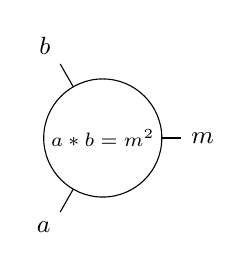
\begin{tikzpicture}[font=\small]
\draw(0,0)circle(.75);\draw(-.375,.65)--(-.54,.94)node[above left]{$b$};\draw(-.375,-.65)--(-.54,-.94)node[below left]{$a$};\draw(.75,0)--(1,0)node[right]{$m$};\node[font=\scriptsize]at(0,0){$a*b=m^2$};
\end{tikzpicture}
\end{center}
\item Giả sử ta có các phần tử $q_1\in Q'(C_1)$, $q_2\in Q'(C_2)$ và $q_3\in Q'(C_3)$ sau:
\begin{center}\ctsevenwirethree{$a*b=m^2$}{$c^2=n^3$}{$m+n=z$}\end{center}
Cho sơ đồ nối dây $G:(C_1,C_2,C_3)\to D$ được vẽ ở đây,
% Source: printed p. 467; PDF p. 476
\begin{center}\ctsevenwireexample{$a*b=m^2$}{$c^2=n^3$}{$m+n=z$}\end{center}
$G(q_1,q_2,q_3)\in Q'(D)$ là gì?
\nobreak\hfill$\diamond$
\end{enumerate}

\noindent\textit{Lời giải 7.4.2.13.}\keepwithnext
\begin{enumerate}[label=\alph*.]
\item Trước hết, $Q'(C_1)$ là gì? Nhắc lại từ Ví dụ~7.4.2.7 rằng $S:\mathcal R\to\mathbf{Sets}$ là đại số các tập con. Ta có:\ctsevennote{Nguyên bản viết ``$S(\mathbb Z^C)\cong\mathbb P(\mathbb Z^3)$''. Nhưng $C=C_1\sqcup C_2\sqcup C_3$ có tám phần tử, trong khi $C_1=\{a,b,m\}$ có ba. Đối số đang tính là $Q'(C_1)$, nên bản dịch sửa số mũ $C$ thành $C_1$.}
\[
Q'(C_1)=S\circ Q(C_1)=S(\mathbb Z^{C_1})\cong\mathbb P(\mathbb Z^3).
\]
Nói cách khác, $q_1\in Q'(C_1)$ phải là một tập con của $\mathbb Z^3$. Hình chỉ ra rằng tập con cần tìm là:\ctsevennote{Nguyên bản viết điều kiện ``$a*b=m$'', nhưng cả ba hình có $q_1$ và quan hệ ở phần~(b) đều ghi $a*b=m^2$. Bản dịch bổ sung số mũ $2$ để đúng phần tử mà hình ở đề bài biểu diễn.}
\[
q_1=\{(a,b,m)\in\mathbb Z^3\mid a*b=m^2\}.
\]
\item Theo các lập luận toán học, ta được một tình huống tương tự Bài tập~7.4.2.11 và câu trả lời cũng tương tự. Cụ thể, $G(q_1,q_2,q_3)$ là tập con sau:
\[
\begin{aligned}
G(q_1,q_2,q_3)=\{(a,c,z)\mid\exists b,m,n\text{ sao cho}\qquad\\
a*b=m^2,\ m+n=z,\ c^2=n^3\}.
\end{aligned}
\]
\nobreak\hfill$\blacklozenge$
\end{enumerate}

\noindent\textit{Ứng dụng 7.4.2.14.}\keepwithnext
Trong khoa học thần kinh nhận thức hoặc kinh tế học công nghiệp, ta có thể muốn hiểu hành vi của một thực thể như tâm trí, xã hội hoặc doanh nghiệp thông qua cấu trúc của nó. Biết mẫu kết nối (bản đồ kết nối thần kinh, chuỗi cung ứng) giữa các thực thể con sẽ giúp hiểu những thay đổi lớn được sinh ra từ những thay đổi nhỏ như thế nào.
\hfill$\diamond\diamond$

% Source: printed p. 468; PDF p. 477
\noindent\textit{Ứng dụng 7.4.2.15.}\keepwithnext
Trong~[36], Radul và Sussman bàn về các \emph{mạng lan truyền}. Có lẽ có thể hiểu cách triển khai của họ theo sơ đồ nối dây và đại số các quan hệ của chúng.
\unskip\nobreak\hfill\mbox{$\diamond\diamond$}\par

% Source: printed p. 469; PDF p. 478
\clearpage
\begin{figure}[p]
\centering
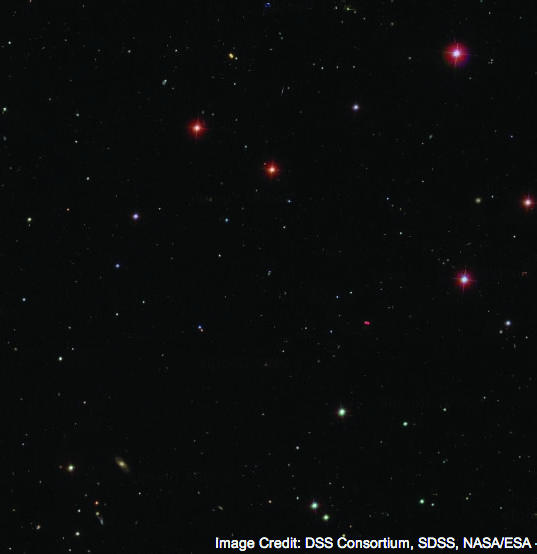
\includegraphics[width=.46\textwidth]{../translation/assets/ch07-sky-view-1.jpg}\hfill
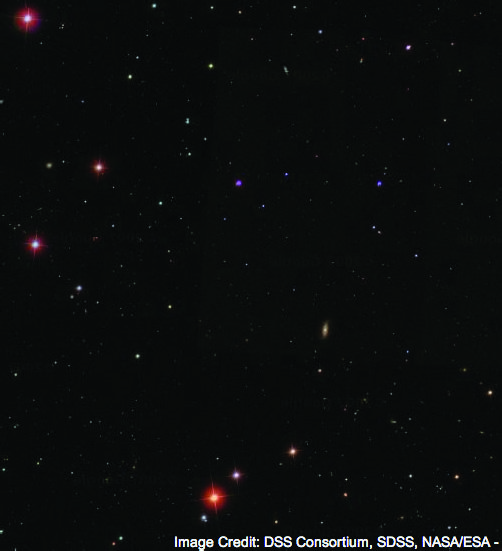
\includegraphics[width=.46\textwidth]{../translation/assets/ch07-sky-view-2.jpg}\\[1ex]
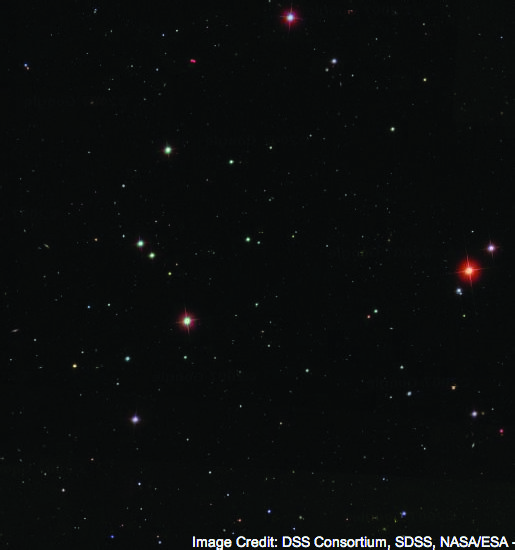
\includegraphics[width=.46\textwidth]{../translation/assets/ch07-sky-view-3.jpg}
\setcounter{figure}{0}
\caption{Ba khung nhìn chồng lên nhau của bầu trời đêm. Nguồn: NASA, ESA, Digitized Sky Survey Consortium.}
\label{fig:ctseven-sky-views}
\end{figure}
\clearpage
% Source: printed p. 470; PDF p. 479
\begin{figure}[p]
\centering
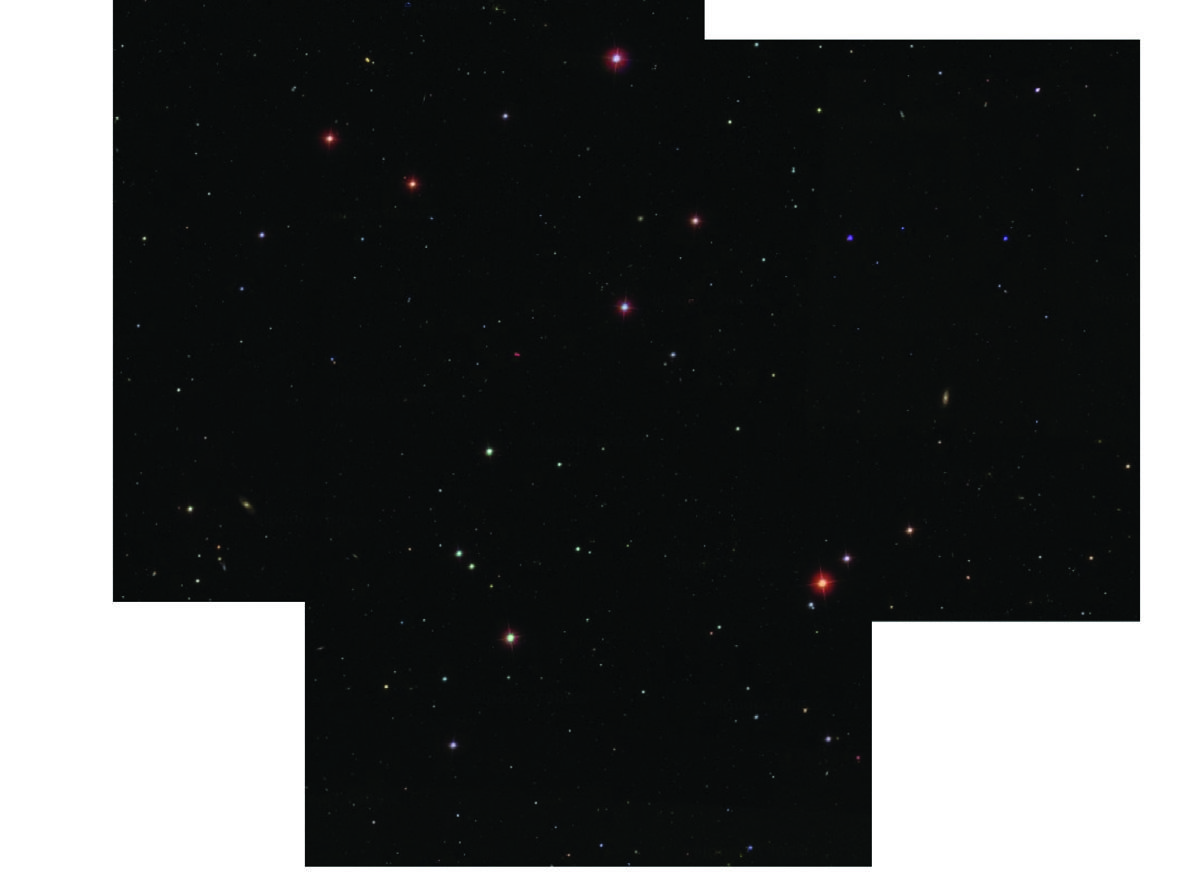
\includegraphics[width=.8\textwidth]{../translation/assets/ch07-sky-glued.jpg}
\setcounter{figure}{1}
\caption{Ba khung nhìn chồng lên nhau đã được ghép thành một khung nhìn nhất quán.}
\label{fig:ctseven-sky-glued}
\end{figure}
\clearpage
